\documentclass[a4paper]{article}

\usepackage[T1]{fontenc}
\usepackage{url}
\usepackage{hyperref}
\usepackage{geometry}
\usepackage{paralist}
\usepackage{graphicx}
\usepackage[cache]{minted}
\newminted{clojure}{fontsize=\fontsize{8}{8},linenos,numbersep=3pt}
\newmintinline{clojure}{fontsize=\fontsize{8}{8}}
\newmintinline{java}{fontsize=\fontsize{8}{8}}
\newmintinline{xml}{fontsize=\fontsize{8}{8}}
\newmintinline{c}{fontsize=\fontsize{8}{8}}
\newmintedfile{java}{frame=lines,fontsize=\fontsize{8}{8},linenos,numbersep=3pt}
\newmintedfile{csharp}{frame=lines,fontsize=\fontsize{8}{8},linenos,numbersep=3pt}
\newmintedfile{cpp}{frame=lines,fontsize=\fontsize{8}{8},linenos,numbersep=3pt}
\newmintedfile{c}{frame=lines,fontsize=\fontsize{8}{8},linenos,numbersep=3pt}
\newmintedfile{xml}{frame=lines,fontsize=\fontsize{8}{8},linenos,numbersep=3pt}
\newcommand{\code}{\clojureinline}


\title{Solving the TTC FIXML Case with FunnyQT}
\author{Tassilo Horn\\
  \href{mailto:horn@uni-koblenz.de}{horn@uni-koblenz.de}}

\begin{document}
\maketitle

\begin{abstract}
  FunnyQT is a model querying and model transformation library for the
  functional Lisp-dialect Clojure providing a rich and efficient querying and
  transformation API.  This paper describes the FunnyQT solution to the TTC
  2014 FIXML transformation case.  It solves the core task of generating Java,
  C\#, and C++ code for a given FIXML message.  It also solves the extension
  tasks of determining reasonable types for the fields of classes, and it
  generates non-object-oriented C code as well.
\end{abstract}


\section{Introduction}
\label{sec:introduction}

This paper describes a solution of the TTC 2014 FIXML
Case~\cite{fixml-case-desc} which solves the core task of generating Java, C\#,
and C++ code for a given FIXML messages.  It also solves the extension task of
heuristically determining appropriate types for the fields of the generated
classes.  Furthermore, the extension task to generate non-object-oriented C
code has been solved as well.  The solution project is available on
Github\footnote{\url{https://github.com/tsdh/ttc14-fixml}}.

The solution is implemented using FunnyQT~\cite{Horn2013MQWFQ} which is a model
querying and transformation library for the functional Lisp dialect
Clojure\footnote{\url{http://clojure.org}}.  Queries and transformations are
plain Clojure programs using the features provided by the FunnyQT API.  This
API is structured into several task-specific sub-APIs/namespaces, e.g., there
is a namespace \emph{funnyqt.polyfns} containing constructs for writing
polymorphic functions dispatching on metamodel type, a namespace
\emph{funnyqt.model2model} containing constructs for model-to-model
transformations, a namespace \emph{funnyqt.bidi} containing constructs for
bidirectional transformations, and so forth.

As a Lisp dialect, Clojure provides strong metaprogramming capabilities that
are exploited by FunnyQT in order to define several \emph{embedded
  domain-specific languages} (DSL, \cite{book:Fowler2010DSL}) for different
tasks.  For example, the pattern matching, in-place transformation,
model-to-model transformation, and bidirectional model transformation
constructs are provided in terms of a small, task-oriented DSL each.

FunnyQT currently supports querying and transforming
EMF~\cite{Steinberg2008EEM} and
JGraLab\footnote{\url{http://jgralab.uni-koblenz.de}} TGraph models, and
support for other modeling frameworks can be added without touching FunnyQT's
internals.  For both EMF and JGraLab, there is one FunnyQT core namespace
(i.e., \emph{funnyqt.emf} and \emph{funnyqt.tg}) providing functions for
accessing and manipulation models of that kind using the framework's
terminology and giving access to any feature provided by that framework.  These
core namespaces are complemented by a namespace \emph{funnyqt.generic} which
provides functions for functionality available on all frameworks in a generic,
framework-agnostic manner.


\section{Solution Overview}
\label{sec:solution-overview}

Before digging into implementation details, here is a brief overview of the
features of the FunnyQT solution.

\begin{compactenum}
\item For every tag name occuring in the XML document, a data type of the same
  name is generated.  For Java, C\#, and C++ the data type is a class, for C
  the data type is a struct.
\item The generated classes/structs contain one field for each XML attribute
  declared for at least one of the corresponding XML elements.  The field type
  is chosen heuristically based on the XML attribute values.  Possible types
  are timestamps, 32 bit integers, 64 bit integers, floating point numbers, and
  strings, each represented by a matching concrete type available in the
  respective programming language.  For timestamps which have no literal
  representation in all four languages, custom parse methods are generated to
  create a timestamp object from a string.
\item The generated classes/structs contain one field per XML tag of which
  child elements occur in at least one XML element.  If a child of a given tag
  occurs at most once, the field's type is of the corresponding class/struct
  (or pointers to that in the case of C++ and C).  If a child of a given tag
  occurs multiple times in at least one element, then the field's type is an
  array of the corresponding class/struct (or a pointer array in the case of
  C++ and C).
\item The generated classes/structs contain one field with name \code|Content|
  if at least one of the corresponding XML elements contains character
  contents.  The type of the field is again chosen heuristically based on those
  text contents.
\item The generated classes contain one default constructor which initializes
  all fields with (one of) the corresponding XML attribute values.  Fields that
  have another class as type are initalized by calling the default constructor
  of that class.  Fields that are arrays of some other class are initialized
  with the maximum number of objects of that class that occur in one single XML
  element.  Each object is initialized with the default constructor.

  Since there are no constructors for C structs, the generated C code contains
  a function \cinline|Str* make_default_Str()| for any struct \cinline|Str|
  instead.
\item The generated classes contain one constructor that has parameters for
  initializing all of its fields.  In the C code, there's one function
  \cinline|Str* make_Str(...)| instead.
\item The generated C++ classes contain a \emph{destructor} that deletes all
  pointer and array-pointer typed fields.  Likewise, for each struct in the C
  code there is a function \cinline|void free_Str(Str* sp)| that recursively
  calls the freeing functions of nested struct pointers and arrays of struct
  pointers.
\item The generated code is pretty idiomatic in all four languages.  That is,
  \begin{compactitem}
  \item for Java and C\#, there is \emph{one source code file per class},
  \item for C++ and C, there is \emph{one header file} and \emph{one
      implementation file} for each class/struct,
  \item for C++ and C, \emph{headers have proper include guards},
  \item \emph{proper import/using statements} are generated for Java and C\#,
    and similarly proper \emph{proper include preprocessor instructions} are
    generated for C++ and C,
  \item the Java classes are defined in a \emph{package corresponding to the
      XML file name},
  \item the C\# and C++ classes are placed in a \emph{namespace corresponding
      to the XML file name},
  \item for Java and C++, every class has a \emph{getter/setter pair} for each
    field,
  \item and for C\# every field is declared with \emph{public auto-implemented
      get and set properties}.
  \item for Java and C++ all \emph{fields are private} while the \emph{getters,
      setters, constructors, and destructors are public},
  \end{compactitem}
\item To ensure \emph{static correctness} (wrt. syntax and typing) of the
  generated code, it is \emph{compiled}, and in the case of C\#, C++, and C
  \emph{linked together in a library} ready to be used.
\item The transformation allows to create a data model given a single FIXML
  message as requested by the case description, but it can also be \emph{run on
    arbitrary many FIXML messages at once}.  The idea is that with a reasonable
  large number of sample FIXML messages, the transformation is able to produce
  a much more accurate data model.  By having more samples, optional attributes
  and child elements are more likely to be identified.  Similarly, child
  elements which usually occur only once but may in fact occur multiple times
  are more likely to be identified and lead to the declaration of a
  corresponding array-valued field instead of just an object-valued field.  And
  finally, the heuristical detection of an appropriate field type benefits from
  more sample data, too.

  Therefore, running the \code|generate_code_and_compile.sh| script of the
  solution project runs the transformation once for each message separately,
  and then again for all messages at once.  In addition to the provided test
  cases, we have added several other FIXML documents available on the web.
\end{compactenum}

Section~\ref{sec:posrpt} in the appendix on page~\pageref{sec:posrpt} shows the
Java, C\#, and C++ classes as well as the C structs and functions that are
generated for the FIXML position report message \texttt{test2.xml}.  It might
be a good idea to have a look at that first before digging into the solution
description.


\section{Solution Description}
\label{sec:solution-description}

In this section, the complete transformation specifications for the core and
extension tasks are going to be explained.  In the listings given in the
following, all function calls are shown in a namespace-qualified form to make
it explicit in which namespace those functions are defined.  Clojure allows to
define short aliases for used namespaces in order to allow qualification while
still being concise.  Table~\ref{tab:namespaces} gives an overview of all
namespaces used by the solution, and the aliases used for accessing them.

\begin{table}[h!t]
  \centering
  \begin{tabular}{| l | l | l |}
    \hline
    \textbf{Alias} & \textbf{Namespace}           & \textbf{Description}\\
    \hline
    \textsf{emf}   & \textsf{funnyqt.emf}         & Core EMF API\\
    \textsf{gen}   & \textsf{funnyqt.generic}     & Generic model access functions\\
    \textsf{io}    & \textsf{clojure.java.io}     & File IO functions\\
    \textsf{m2m}   & \textsf{funnyqt.model2model} & Model-to-Model transformation API\\
    \textsf{oo}    & \textsf{ttc14-fixml.oo}      & Generated OO model API\\
    \textsf{poly}  & \textsf{funnyqt.polyfns}     & Polymorphic function API\\
    \textsf{s}     & \textsf{stencil.core}        & The Stencil templating library\\
    \textsf{str}   & \textsf{clojure.string}      & String utility functions\\
    \textsf{tg}    & \textsf{funnyqt.emf}         & Core TGraph API\\
    \textsf{u}     & \textsf{funnyqt.utils}       & Utility functions (e.g., error handling)\\
    \textsf{xml}   & \textsf{ttc14-fixml.xml}     & Generated XML model API\\
    \textsf{xmltg} & \textsf{funnyqt.xmltg}       & Generic XML to XML-Graph transformation\\
    \hline
  \end{tabular}
  \caption{Used Clojure and FunnyQT namespaces with their aliases}
  \label{tab:namespaces}
\end{table}

All function calls that are not qualified with an alias are calls to functions
in the \emph{clojure.core} namespace which is available in any other namespace
by default.

\subsection{XML to Model}
\label{sec:xml2model}

Since handling XML files is a common task, FunnyQT already ships with a
namespace \emph{funnyqt.xmltg} which contains a transformation from XML files
to a DOM-like TGraph model conforming to the metamodel in
Figure~\ref{fig:xml-mm}.

\begin{figure}[h!t]
  \centering
  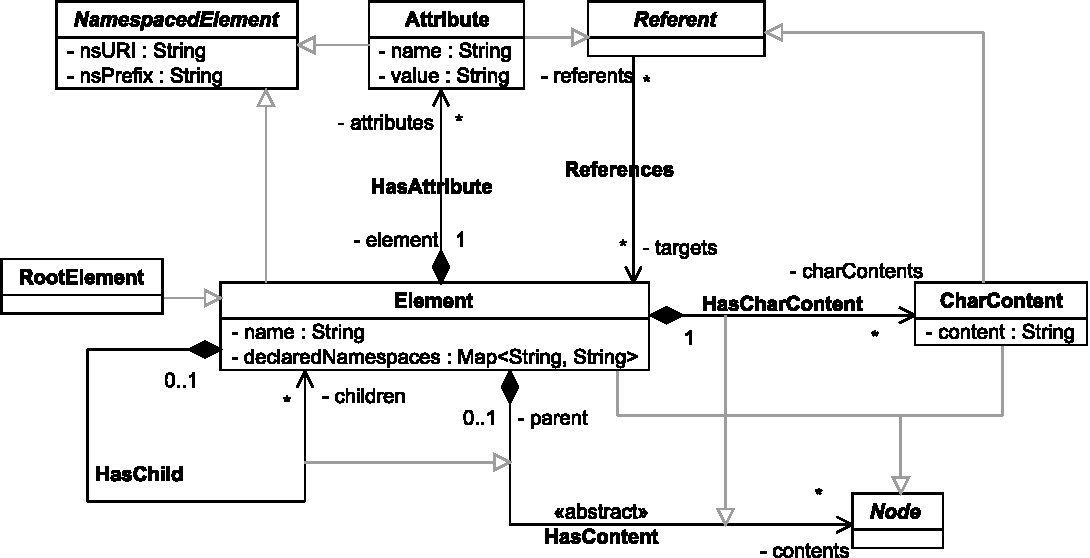
\includegraphics[width=.8\textwidth]{xml-schema}
  \caption{FunnyQT's XML Graph metamodel}
  \label{fig:xml-mm}
\end{figure}

It models XML elements, their attributes, text contents, and children.  It also
supports XML namespaces, and the transformation may be supplemented with
additional XML schema information in order to resolve \texttt{IDREF} and
\texttt{IDREFS} references automatically.

\begin{sloppypar}
  Namespaces and references are not important in this case, so a plain call
  \code|(xmltg/xml2xml-graph "test2.xml")| suffices to handle core task
  number~1, i.e., generate an XML model from an XML file.  The graph
  corresponding to the position report message contained in the file
  \texttt{test2.xml} is visualized in the appendix
  Section~\ref{sec:posrpt:xml}.
\end{sloppypar}

The \code|xml2xml-graph| function uses Java's \emph{Stream API for XML}
(\emph{StAX}) under the hoods, so XML files that aren't well-formed lead to
parsing errors.  These are the errors you get for the invalid test files
\texttt{test7.xml} and \texttt{test8.xml}:

\begin{clojurecode*}{numbers=none}
(xmltg/xml2xml-graph "messages/test7.xml")
;NoSuchElementException ParseError at [row,col]:[14,7]
;Message: The element type "Sndr" must be terminated by the matching end-tag "</Sndr>".
(xmltg/xml2xml-graph "messages/test8.xml")
;NoSuchElementException ParseError at [row,col]:[19,9]
;Message: The element type "Hdr" must be terminated by the matching end-tag "</Hdr>".
\end{clojurecode*}


\subsection{XML Model to OO Model}
\label{sec:xml-to-oo}

Core task~2 deals with transforming the XML models generated by core task~1
into models conforming to a metamodel suited for object-oriented programming
languages.  The metamodel used by the FunnyQT solution is shown in
Figure~\ref{fig:oo-mm}.

\begin{figure}[h!t]
  \centering
  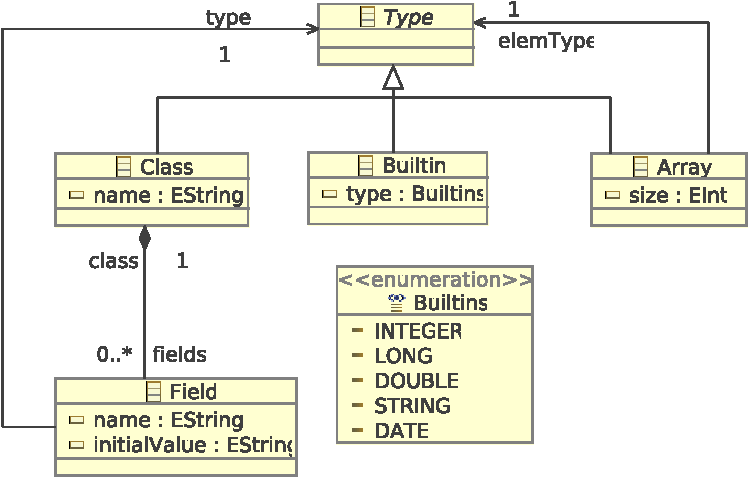
\includegraphics[width=.6\textwidth]{../model/oo}
  \caption{The OO metamodel}
  \label{fig:oo-mm}
\end{figure}

Classes have a name and arbitray many fields.  Each field has a name, an
initial value, and a type.  Types may be classes, builtin types, or arrays.
The different builtin types will be used for solving the extension task of
determining a sensible type for a field, and instead of creating many separate
fields if an XML element contains multiple child elements with a given tag, we
create just one field which is an array of the class corresponding to the child
element's tag name.

The metamodel in Figure~\ref{fig:oo-mm} is an Ecore model, so the
transformation from XML model to OO model actually transforms between two
different modeling frameworks: the input is an XML TGraph model, and the output
is an OO EMF model.

In the remainder of this section, the transformation will be discussed in
details.  Before the actual transformation definition, there's a little bit
helper code.  The following two calls generate metamodel-specific APIs for the
XML and the OO metamodels in the namespaces \code|ttc14-fixml.xml| and
\code|ttc14-fixml.oo| which are referred to by the aliases \code|xml| and
\code|oo|.

\begin{clojurecode}
(tg/generate-schema-functions       "xml-schema.tg"  ttc14-fixml.xml xml)
(emf/generate-ecore-model-functions "model/oo.ecore" ttc14-fixml.oo  oo)
\end{clojurecode}

The generated APIs contain a pair of getter and setter functions for each
attribute (e.g., \code|(xml/name el)| and \code|(xms/set-name! el val)|), role
name accessor functions (e.g., \code|(xml/->children el)| or \code|(oo/fields
cls)|), and several more.

Next, we define some constants for the values of the \code|Builtins|
enumeration of the OO metamodel.

\begin{clojurecode*}{firstnumber=3}
(def DATE    (emf/eenum-literal 'Builtins.DATE))
(def INTEGER (emf/eenum-literal 'Builtins.INTEGER))
(def LONG    (emf/eenum-literal 'Builtins.LONG))
(def DOUBLE  (emf/eenum-literal 'Builtins.DOUBLE))
(def STRING  (emf/eenum-literal 'Builtins.STRING))
\end{clojurecode*}

The EMF-specific function \code|emf/eenum-literal| returns the enumeration
literal given by a symbol denoting its qualified name.

Then, the actual transformation definition from XML model to OO model follows.
In FunnyQT, a model-to-model transformation is specified using the
\code|m2m/deftransformation| macro.  It receives the name of the transformation
(\code|xml-graph2oo-model|), and a vector defining input models and output
models plus additional parameters.  In this case, there is only one single
input model \code|xml|, one single output model \code|oo|, and no additional
parameters.

\begin{clojurecode*}{firstnumber=8}
(m2m/deftransformation xml-graph2oo-model [[xml] [oo]]
  ;; rule & function definitions...
  )
\end{clojurecode*}

Inside such a transformation definition, arbitrary many rule and helper
function definitions may occur.  The first rule of the transformation is
\code|element2class| shown in the next listing.

\begin{clojurecode*}{firstnumber=9}
  (^:top element2class
   :from [e '[:and Element !RootElement]]
   :to   [c (element-name2class (xml/name e))])
\end{clojurecode*}

The \code|^:top| annotation defines this rule as a top-level rule.  Such a rule
is automatically applied to all matching elements.  The \code|:from| clause
restricts the elements \code|e| this rule is applicable for to those that are
of metamodel type \code|Element| but not of type \code|RootElement| (which is a
subclass of \code|Element| according to Figure~\ref{fig:xml-mm}).  The reason
is that we don't want to create a class for the \texttt{FIXML} element which is
the root element of any FIXML message.

The \code|:to| clause defines which elements should be created for matching
elements.  Usually, it would be specified as \code|:to [x 'SomeClass]| in which
case \code|x| would be a new element of type \code|SomeClass|.  However, in the
current case, there is no one-to-one mapping between XML elements and OO
classes, because the XML model may contain multiple elements with the same tag
name, and there should be exactly one OO class per unique tag name.  Therefore,
the \code|:to| clause delegates the creation of class \code|c| to another rule
\code|element-name2class| providing \code|e|'s tag name as argument.

The semantics of a rule are as follows.  When it is applied to an input element
for which its \code|:from| clause matches, target elements are created
according to its \code|:to| cause.  The mapping from input to output elements
is saved.  When a rule gets applied to an element it has already been applied
to, the elements that have been created by the first call are returned instead
of creating new elements.  That way, calling a rule serves both creation of
target elements as well as resolution of input to output elements in terms of
traceability.

The next rule is \code|element-name2class| which is shown below.

\begin{clojurecode*}{firstnumber=12}
  (element-name2class
   :from [tag-name]
   :to   [c 'Class {:name tag-name}]
   (doseq [[an at av] (all-attributes tag-name)]
     (attribute2field an at av c))
   (doseq [[tag max-child-no] (all-children tag-name)]
     (children-of-same-tag2field tag max-child-no c))
   (when-let [char-conts (seq (all-character-contents tag-name))]
     (character-contents2field char-conts c)))
\end{clojurecode*}

This rule receives as input a plain string, the \code|tag-name| of an element,
and it creates a \code|Class c| in the target model.  The name of the class
corresponds to the \code|tag-name|.  According to the rule semantics sketched
above and the fact that this rule gets called with the tag name of any element
by \code|element2class|, there will be one target class for every unique tag
name.

Following the \code|:from| and \code|:to| clauses comes the rule's body where
arbitrary code may be written.  Here, three other rules \code|attribute2field|,
\code|children-of-same-tag2field|, and \code|character-contents2field| are
called for all XML attributes, child elements, and character
contents\footnote{The case description doesn't specify if and how XML character
  content should be handled.  However, without them transforming
  \texttt{test3.xml} and \texttt{test4.xml} would lead to classes with no
  fields at all which doesn't make much sense.}  of element \code|e|,
respectively.  These rules are shown below.

\begin{clojurecode*}{firstnumber=21}
  (attribute2field
   :from [an at av class]
   :to   [f 'Field {:name an :type at :initialValue av :class class}])
  (children-of-same-tag2field
   :from [tag max-child-no class]
   :to   [f 'Field {:class class}]
   (if (= 1 max-child-no)
     (do (oo/set-name! f (str tag "_obj"))
         (oo/->set-type! f (element-name2class tag)))
     (let [array-type (oo/create-Array! oo :size max-child-no :elemType (element-name2class tag))]
       (oo/set-name! f (str tag "_objs"))
       (oo/->set-type! f array-type))))
       (oo/->set-type! f array-type))))
  (character-contents2field
   :from [char-conts class]
   :to   [f 'Field {:name "Content" :initialValue (first char-conts)
                    :type (guess-type char-conts) :class class}])
\end{clojurecode*}

The \code|attribute2field| rule gets an attribute name \code|an|, its type
\code|at|, its initial value \code|av|, and the \code|class| to which to add
the new field \code|f|.

The \code|children-of-same-tag2field| rule gets a child tag name \code|tag|,
the maximum number of children having that tag \code|max-child-no|, and again
the \code|class| to which to add the new field \code|f|.  If there is only one
child of a tag, then the field's type is the class corresponding to the
tag\footnote{Note how the rule \code|element-name2class| is called here to
  resolve the class created for a tag name}.  If there are multiple children of
that tag, then the field's type is array of objects of the class corresponding
to the tag.

Lastly, \code|character-contents2field| receives a collection \code|char-conts|
of character contents and again the \code|class| to which to add the new field
\code|f|.  That new field gets the fixed name ``Content'', and its type is
guessed by a function \code|guess-type| which is shown in the next listing.

\begin{clojurecode*}{firstnumber=38}
  (guess-type [vals]
   (let [ts (set (map #(condp re-matches %
                         #"\d\d\d\d-\d\d-\d\d.*" DATE
                         #"[+-]?\d+\.\d+"        DOUBLE
                         #"[+-]?\d+"             (int-type %)
                         STRING) vals))]
     (get-or-create-builtin-type
      (cond
       (= (count ts) 1)              (first ts)
       (= ts #{DOUBLE INTEGER})      DOUBLE
       (= ts #{DOUBLE LONG})         DOUBLE
       (= ts #{DOUBLE LONG INTEGER}) DOUBLE
       (= ts #{INTEGER LONG})        LONG
       :else                         STRING))))
  (int-type [val]
   (try (and (Integer/parseInt val) INTEGER)
        (catch NumberFormatException _
          (try (and (Long/parseLong val) LONG)
               (catch NumberFormatException _
                 STRING)))))
  (get-or-create-builtin-type
   :from [t]
   :to   [bit 'Builtin {:type t}])
\end{clojurecode*}

The \code|guess-type| function receives a collection \code|vals| from which to
guess an appropriate type.  \code|vals| could either be all character contents
of an XML element, or all attribute values of an attribute that occurs in many
XML elements of the same tag.

Every given value is checked against a regular expression that determines its
type being either a timestamp in ISO 8601 notation, a double value, or an
integer value.  If neither matches, then \code|STRING| is used as its type.  In
case of an integer value, the function \code|int-type| further determines if
the value can be represented as a 32 bit integer, or if a 64 bit long is
needed, or if it is so large that it can only be represented as a string.

Lines 45 to 51 pick the type that can be used to represent all values.  If all
values are guessed to be of the very same type (line 46), then this type is
chosen.  For multiple numeric types, the respective ``largest'' type is chosen
where \code|INTEGER| \(<\)
\code|LONG| \(<\) \code|DOUBLE|.  Else, we fall back to \code|STRING|.

The picked type is then passed to the rule \code|get-or-create-builtin-type|
which creates a \code|Builtin| whose \code|type| attribute is set to the picked
type \code|t|.  As a result, the OO model contains at most one \code|Builtin|
element per \code|Builtins| enumeration literal.

The last part of the transformation are the functions that compute the
information about attributes, child elements, and character contents that are
passed to the respective rules by the \code|element-name2class| rule starting
in line~12.  All three functions have to cater for the fact that elements of
the same tag may occur multiple times in the XML document, and each occurence
may use a different subset of the attributes and child elements it may have
according to the FIXML specification.  Therefore, a helper function
\code|elements-of-tag| is defined that given a \code|tag-name| returns all
elements having that tag.

\begin{clojurecode*}{firstnumber=61}
  (all-attributes [tag-name]
   (->> (elements-of-tag tag-name) (mapcat xml/->attributes) (group-by xml/name)
        (map (fn [[an as]]
               [an (guess-type (map xml/value as)) (xml/value (first as))]))))
  (elements-of-tag [tag-name]
   (->> (xml/vseq-Element xml) (filter #(= tag-name (xml/name %)))))
  (all-children [tag-name]
   (let [child-tag-names (->> (elements-of-tag tag-name) (mapcat xml/->children)
                              (map xml/name) (into #{}))]
     (map (fn [ctn] [ctn (max-children-of-tag tag-name ctn)]) child-tag-names)))
  (max-children-of-tag [tag-name child-tag-name]
   (reduce (fn [old el]
             (let [cot (count (filter #(= child-tag-name (xml/name %)) (xml/->children el)))]
               (if (> cot old) cot old)))
               0 (elements-of-tag tag-name)))
  (all-character-contents [tag-name]
   (->> (elements-of-tag tag-name) (mapcat xml/->charContents)
        (map xml/content) (remove str/blank?))))
\end{clojurecode*}

\code|all-attributes| gets a \code|tag-name|, computes all elements having this
tag, computes the union of attributes, and groups them by their name.  This
results in a sequence of tuples of the form \code|[an as]| where \code|an| is
the attribute name and \code|as| is a collection of all attributes with that
name.  All those tuples are then processed with a function that returns a tuple
of the attribute name, the type guessed from all values, and the first
attribute's value (which will be used as initial value for the corresponding
field).  That's exactly the information relevant for the \code|attribute2field|
rule (see call in line~16 and definition starting in line~21).

\code|all-children| first computes the tag names of all elements that occur as
child of an element with tag \code|tag-name|.  For each of them, it computes a
tuple of the form \code|[ctn max-child-no]| where \code|ctn| is the child tag
name, and \code|max-child-no| is the largest number of children of that child
tag that occur together in an element.  Again, that's the relevant information
for the \code|children-of-same-tag2field| rule (see call in line~18 and
definition starting in line~24)

Lastly, \code|all-character-contents| returns a sequence containing all
non-empty character contents of all elements of tag \code|tag-name|.  Its
result is passed to the \code|character-contents2field| rule (called in line~20
and defined in line~34).

The OO model generated for the the position report message contained in the
file \texttt{test2.xml} is visualized in the appendix
Section~\ref{sec:posrpt:oo}.

\subsection{OO Model to Code}
\label{sec:oo-model-to-code}

The third and last step of the overall transformation is to generate code in
different programming languages from the OO model created in the previous step.
In addition to the core task languages, the FunnyQT solution also generates C
code as an extension.

One crucial benefit of FunnyQT being a Clojure library is that we can simply
use arbitrary other Clojure and Java libraries for our needs.  So for this
task, we use the excellent
\emph{Stencil}\footnote{\url{https://github.com/davidsantiago/stencil}}
library.  Stencil is a Clojure templating library implementing the popular,
lightweight \emph{Mustache}
specification\footnote{\url{http://mustache.github.io/}}.  The idea of Mustache
is that one defines a template file containing placeholders which can be
rendered to a concrete file by providing a map where the keys are the
placeholder names and the values are the text that should be substituted.
There are also placeholders for collections in which case the corresponding
value of the map has to be a collection of maps.

We'll discuss the solution using the template for Java.

\javafile{../resources/templates/class.java}

When we want to render a class named \code|C| in package \code|p| that uses the
\code|java.util.Date| class and contains two fields \code|f1| and \code|f2| of
type \code|String| and \code|Date| and initial values ``Hello'' and
\code|2003-09-10T00:00:00|, we would need to provide the following map to the
rendering function.

\begin{clojurecode*}{linenos=none}
  {:pkg-name "p"
   :imports [{:imported-class "java.util.Date"}]
   :class-name "C"
   :fields [{:field-type "String"
             :field-name "f1"
             :field-value-exp "\"Hello\""
             :first true}
            {:field-type "Date"
             :field-name "f2"
             :field-value-exp "Util.parseDate(\"2003-09-10T00:00:00\");"}]}
\end{clojurecode*}

The \code|:first| key with value \code|true| needs to be added to the map
corresponding to the first field of the class for rendering the parameter list
of the non-default constructor.  Every parameter which has no \code|:first| key
gets prepended by a comma and a space\footnote{See line 26 of the template
  which uses an inverted mustache section: \javainline|{{^first}}, {{/first}}|.
  Only if there is no \code|:first| key (or a \code|:first| key with value
  \code|false|) the comma followed by a space is emitted.}.

The templates for the other languages use the same keys\footnote{The key names
  are a bit Java specific, but they have analogues in the other languages.  For
  example, for C and C++ the \code|:imported-class| values in the
  \code|:imports| vector are in fact the header files to be included.}, so the
essential job of the code generation task is to derive such a map for every
class in our OO model that can then be passed to Stencil's rendering function.

This is done using a FunnyQT polymorphic function \code|to-mustache| whose
definition is given below.

\begin{clojurecode}
(poly/declare-polyfn to-mustache [el lang pkg])

(poly/defpolyfn to-mustache oo.Class [cls lang pkg]
  {:pkg-name pkg
   :imports (get-imports cls lang)
   :class-name (oo/name cls)
   :fields (mark-first-field (map #(to-mustache % lang pkg) (oo/->fields cls)))})

(poly/defpolyfn to-mustache oo.Field [f lang pkg]
  {:field-type (field-type (oo/->type f) lang)
   :field-name (oo/name f)
   :field-value-exp (field-value-exp f lang)
   :uscored-field-name (str "_" (oo/name f))
   :plain-field-type (let [t (oo/->type f)]
                       (gen/type-case t
                         'Array (oo/name (oo/->elemType t))
                         'Class (oo/name t)
                         nil))
   :pointer (gen/has-type? (oo/type f) 'Class)
   :array (gen/has-type? (oo/type f) 'Array)})
\end{clojurecode}

A polymorphic function in FunnyQT is a function that dispatches between several
implementations based on the metamodel type of its first argument.  Thus you
can view them as a kind of object-oriented method attached to metamodel classes
that may be overridden by subclasses.

Line 1 declares the polymorphic function \code|to-mustache| and defines that it
gets three parameters: an OO model element \code|el|, the target language
\code|lang|, and the package/namespace name \code|pkg| in which the
class/struct should be generated.

Lines 3 to 7 then define an implementation for elements of the metamodel class
\code|Class|.  It returns a literal map where \code|:pkg-name| is the package
name provided as argument, \code|:imports| is computed by a function
\code|get-imports|, the \code|:class-name| is the name of the \code|Class|
element \code|cls|, and \code|:fields| is computed by applying the
\code|to-mustache| function to all fields of the class (and marking the first
as discussed above).

Lines 9 to 20 define the \code|to-mustache| implementation for elements of
metamodel class \code|Field|.  The language-dependent \code|:field-type| is
computed by a function \code|field-type|, the \code|:field-name| is the name of
the \code|Field| element, and the \code|:field-value-exp| used to initialize
the field in the default constructor is computed by a function
\code|field-value-exp|.

The additional key \code|:uscored-field-name| is the field name prefixed with
an underscore.  This variant is used for fields in C++ and C\#, because in
these languages, a field must not be named like its enclosing class but there
are FIXML elements that have an attribute named like the element tag, e.g.,
\xmlinline|<Amt Typ="FMTM" Amt="0.00"/>|.

The three further keys \code|:plain-field-type|, \code|:pointer|, and
\code|:array| are only needed for the C and C++ templates where they are used
to generate a proper destructor or a proper function for freeing a struct
pointer recursively.

The next listing shown the \code|field-type| function returning the appropriate
data type name for a given \code|field| when generating code for language
\code|lang|.

\begin{clojurecode*}{firstnumber=21}
(def string-type {:java "String", :csharp "string", :cpp "std::string", :c "char*"})
(def timestamp-type {:java "Date", :csharp "DateTime", :cpp "std::tm", :c "struct tm"})

(defn object-type [class lang]
  (str (oo/name class) (when (#{:c :cpp} lang) "*")))

(defn field-type [type lang]
  (gen/type-case type
    'Class   (object-type type lang)
    'Builtin (condp = (oo/type type)
               DATE    (timestamp-type lang)
               DOUBLE  "double"
               INTEGER "int"
               LONG    "long"
               STRING  (string-type lang))
    'Array   (str (field-type (oo/->elemType type) lang)
                  (if (#{:c :cpp} lang) "*" "[]"))))
\end{clojurecode*}

In case the field's type is a class, that classes' name is used.  In the case
of C and C++, an asterisk is prepended, because there pointers to that class
are used.

The builtin numeric types have the same name in all four languages, but for
dates and strings, a distinction has to be made.  Lines 21 and 22 simply define
constant maps from language keys to appropriate type names.  In Clojure, a map
is a function of its keys, so \code|(string-type :cpp)| returns
\code|"std::string"| for example.

In the case the field's type is an array, the array's element type name gets
prepended with either an asterisk (for C and C++) or a pair of brackets (Java
and C\#).

The probably most complex function of the code generation is
\code|field-value-exp| shown in the next listing.  It generates the expression
used to initialize the given \code|field| in the programming language
\code|lang|.

\begin{clojurecode*}{firstnumber=38}
(defn field-value-exp [field lang]
  (let [type (oo/->type field)
        val (oo/initialValue field)]
    (gen/type-case type
      'Class (if (= lang :c)
               (str "make_default_" (oo/name (oo/->type field)) "()")
               (str "new " (oo/name (oo/->type field)) "()"))
      'Builtin (condp = (oo/type type)
                 DATE   (case lang
                          :cpp (str "Util::parseDate(\"" val "\")")
                          :c   (str "parseDate(\"" val "\")")
                          (str "Util.parseDate(\"" val "\")"))
                 STRING (str "\"" val "\"")
                 LONG   (str val "L")
                 val)
      'Array (if (= lang :c)
               (format "(%s) make_pointer_array(%s, %s)"
                       (field-type type lang)
                       (oo/size type)
                       (str/join ", " (for [i (range (oo/size type))]
                                        (format "make_default_%s()"
                                                (oo/name (oo/->elemType type))))))
               (format "new %s[%s] {%s}"
                       (field-type (oo/->elemType type) lang)
                       (if (= lang :cpp) (oo/size type) "")
                       (str/join ", " (for [i (range (oo/size type))]
                                        (format "new %s()"
                                                (oo/name (oo/->elemType type))))))))))
\end{clojurecode*}

Fields that have some other class as their type, the value expression is
usually \code|new OtherClass()|, i.e., a call to that class' default
constructor.  In C, however, there is no \code|new| and no constructors, so the
C template generates a \code|make_default_StructName()| function for which a
call is returned here.

For fields of builtin types several distinctions have to be made.  Dates are
always parsed by an auxilliary \code|parseDate()| method contained by some
\code|Util| class.  Strings have to be enclosed in double quotes.  Long
literals need to be suffixed with \code|L|, else a long literal that's larger
than the largest integer will lead to a parsing error.  Lastly, integer and
double numbers can be emitted as-is, i.e., as they occured in the XML document.

For array fields, the value expression is usually a literal array initializer
form containing calls to the default constructors of the class corresponding to
the array's element type.  Again, since there's no \code|new| and no
constructors in C, a call to a generic \code|make_pointer_array()| varargs
function is generated.  This function allocates memory for a pointer array of
the given size \(n\)
plus one, assigns the pointers given as arguments to the indices \(0\)
to \(n-1\),
and index \(n\)
is set to \cinline|NULL|.  This \cinline|NULL|-termination of the arrays allows
us to generate proper freeing functions that recursively free the memory held
by a struct of the data model.  A possibly better approach was to use some
third-party memory management library like
\emph{talloc}\footnote{\url{http://talloc.samba.org/}} instead which wouldn't
require such ``tricks'', but we decided to only use the standard C library.

The next listing contains the \code|file-ending| function which has
implementations for arity one and two.  If given only a \code|lang| keyword, it
returns the typical file name suffix for that language where for C and C++ it
returns the suffix of a header.  To get the file name ending for the
implementation file instead, one needs to call \code|file-ending| with
additional argument \code|impl| set to \code|true|.

\begin{clojurecode*}{firstnumber=66}
(defn file-ending
  ([lang] ({:java "java", :csharp "cs", :cpp "hpp", :c "h"} lang))
  ([lang impl]
     (if impl
       (case lang :cpp "cpp" :c "c")
       (file-ending lang))))
\end{clojurecode*}

The next listing shows the \code|get-imports| function which calculates the
classes/files/namespaces of a class \code|cls| that need to be
imported/included/used in the language \code|lang|.

\begin{clojurecode*}{firstnumber=72}
(defn get-imports [cls lang]
  (letfn [(includes-from-type [t]
            (gen/type-case t
              'Class   (when (#{:c :cpp} lang)
                         [(format "\"%s.%s\"" (oo/name t) (file-ending lang))])
              'Builtin (condp = (oo/type t)
                         DATE   (case lang
                                    :java   ["java.util.Date"]
                                    :csharp ["System"]
                                    :cpp    ["<ctime>" "\"Util.hpp\""]
                                    :c      ["<time.h>" "\"Util.h\""])
                         STRING (when (= lang :cpp) ["<string>"])
                         nil)
              'Array   (concat (when (#{:c :cpp} lang)
                                 (includes-from-type (oo/->elemType t)))
                               (when (= lang :c)
                                 ["\"Util.h\""]))))]
    (map (fn [import] {:imported-class import})
         (set (mapcat includes-from-type (gen/adjs cls :fields :type))))))
\end{clojurecode*}

In the case of C and C++, every implementation file of a class needs to include
the corresponding header.  Classes that have fields of a date type need to
import special classes/namespaces/headers in all four languages, and for C++,
there needs to be an include even for being able to use the standard string
type.  For arrays, the C and C++ versions need to include the header
corresponding to the element type, and for C also the \texttt{Util.h} header
has to be included because of the call to the generic pointer-array creation
function.

The main driver of the code generation is the function \code|oo2code| given
below.

\begin{clojurecode*}{firstnumber=91}
(defn oo2code [oo pkg lang]
  (let [dir (format "results/%s/%s" (name lang) pkg)]
    (.mkdirs (io/file dir))
    (spit (format "%s/Util.%s" dir (file-ending lang))
          (s/render-file (format "templates/Util.%s" (file-ending lang))
                         {:pkg-name pkg}))
    (when (#{:c :cpp} lang)
      (spit (format "%s/Util.%s" dir (file-ending lang true))
            (s/render-file (format "templates/Util.%s" (file-ending lang true))
                           {:pkg-name pkg})))
    (doseq [cls (oo/eall-Classes oo)]
      (spit (format "%s/%s.%s" dir (oo/name cls) (file-ending lang))
            (s/render-file (format "templates/class.%s" (file-ending lang))
                           (to-mustache cls lang pkg)))
      (when (#{:c :cpp} lang)
        (spit (format "%s/%s.%s" dir (oo/name cls) (file-ending lang true))
              (s/render-file (format "templates/class.%s" (file-ending lang true))
                             (to-mustache cls lang pkg)))))))
\end{clojurecode*}

It the receives the OO model \code|oo|, a package name in which to generate the
code, and the target language \code|lang|.  The files will be generated in a
directory \code|results/<lang>/<pkg>/|.

Lines 94 to 100 generate the utility class file containing the date parsing
methods (for C and C++, split in header and implementation) and the generic
pointer-array creation function in the case of C.

Then, lines 101 to 108 generate a class file for every class contained in the
OO model.  Again, in the case of C and C++, actually one header and one
implementation file is emitted per class.

\section{Evaluation}
\label{sec:evaluation}

\paragraph{Complexity.}
\label{sec:complexity}

The complexity according to the evaluation criteria should be measured as the
sum of number of operator occurrences and feature and entity type name
references in the specification expressions.

The FunnyQT solution contains about 300 expressions (function calls,
conditional expressions, etc.), 24 metamodel type references, and 18 property
references resulting in a complexity of 342.  So it is probably quite complex,
but most of its complexity is a result of that it does much more than what was
required, e.g., guess appropriate field types, generate C code, generate
destructors and freeing functions for C++ and C, separate header and
implementation files for C++ and C, generate getters and setters, etc.


\paragraph{Accuracy.}
\label{sec:accuracy}

Accuracy should measure the degree of syntactical correctness of the generated
code, and the degree of how well the generated code matches the source FIXML
messages.

The FunnyQT solution has a very high accuracy.  The code is correct for all
four languages and compiles without warnings.  It also matches the source FIXML
messages very well.  Especially creating array fields for XML child elements
that occur multiple times is much better than creating numbered fields.  Also,
guessing appropriate types for the fields instead of always using string
improves the usefulness of the generated code.  Finally, that the
transformation can be run on an arbitrarily large sample of FIXML messages in
one go improves the accuracy of the generated classes even more.

\paragraph{Development effort.}
\label{sec:development-effort}

Developing the solution has been a on-and-off effort.  Prototyping an initial
solution only for Java took about 4 person-hours.  Extending that to C\# was
rather easy, however when C++ (and even worse C) with their pointers and split
in headers and implementation files came into play, a major refactoring of the
code generation code was needed.  So all in all, the overall development time
can be estimated with about 12 person-hours.

\paragraph{Fault tolerance.}
\label{sec:fault-tolerance}

Since FunnyQT's generic \code|xml2xml-graph| transformation uses Java's StAX
API internally, the fault tolerance is high.  Documents that are not
well-formed lead to errors like the ones printed in Section~\ref{sec:xml2model}
for the broken test files \texttt{test7.xml} and \texttt{test8.xml}.

If the XML documents also declare or reference a DTD or an XML schema, then the
transformation can also use a validating StAX parser that also throws an
exception when the document while being well-formed does not conform to the
document's schema.


\paragraph{Execution time.}
\label{sec:execution-time}

Table~\ref{tab:exec-times} shows the execution times for the different test
files.  The column \textbf{XML2OO} contains the times for parsing the XML
document and generating an XML graph from it (Section~\ref{sec:xml2model}),
plus the time needed to transform that into an OO model
(Section~\ref{sec:xml-to-oo}).

The columns \textbf{Java}, \textbf{C\#}, \textbf{C++}, and \textbf{C} contain
the time needed to generate code in the respective language from the OO model
(Section~\ref{sec:oo-model-to-code}).

The column \textbf{Overall} is the overall time needed for parsing the XML
document to a graph, transforming that to an OO model, and generating code in
the four languages.

\begin{table}[h!t]
  \centering
  \begin{tabular}{| l | r | r | r | r | r | r |}
    \hline
    \textbf{Message} & \textbf{XML2OO} & \textbf{Java} & \textbf{C\#} & \textbf{C++} & \textbf{C} & \textbf{Overall}\\
    \hline
    \texttt{test1}                    & 9.0   & 7.5  & 7.8  & 15.9 & 13.0 & 54.8\\
    \texttt{test2}                    & 14.9  & 19.1 & 19.8 & 27.0 & 26.8 & 109.2\\
    \texttt{test3}                    & 13.3  & 13.5 & 9.6  & 20.5 & 20.2 & 78.3\\
    \texttt{test4}                    & 21.9  & 12.8 & 9.6  & 22.9 & 21.6 & 90.9\\
    \texttt{test5}                    & 50.7  & 13.6 & 10.2 & 20.6 & 22.2 & 119.2\\
    \texttt{test6}                    & 96.5  & 13.4 & 7.5  & 17.1 & 21.6 & 157.3\\
    \hline
    \texttt{batch\_message}           & 21.1  & 88.3 & 30.8 & 74.0 & 67.3 & 304.2\\
    \texttt{new\_order\_single}       & 9.9   & 12.6 & 10.1 & 22.9 & 22.9 & 81.6\\
    \texttt{trade\_subm\_allocs}      & 18.9  & 5.5  & 5.0  & 10.1 & 9.0  & 49.5\\
    \texttt{trade\_subm\_allocs\_ack} & 21.6  & 7.2  & 7.0  & 14.8 & 19.4 & 71.1\\
    \texttt{trade\_subm\_clearing}    & 17.0  & 6.7  & 7.3  & 14.2 & 12.2 & 58.9\\
    \hline
    All 11 at once                    & 264.5 & 30.1 & 21.3 & 54.3 & 60.2 & 432.0\\
    \hline
  \end{tabular}
  \caption{Execution times for the test FIXML messages (in milliseconds)}
  \label{tab:exec-times}
\end{table}

The FIXML messages \texttt{test1} to \texttt{test6} are the test files provided
in the case
project\footnote{\url{https://github.com/TransformationToolContest/ttc2014-fixml}}.
The next five messages are some additional ones that can be found on the web.
The last line shows the time needed for parsing all 11 FIXML messages into one
XML graph, transforming that to an OO model, and then emitting code for the
four languages.


\paragraph{Modularity.}
\label{sec:modularity}

The \code|xml-graph2oo-model| consists of \(r=6\)
rules, one marked as a top-level rule.  All other rules are called explicitly
which gives \(d=5\)
or \(d=6\)
dependencies, depending on if the marking of a top-level rule counts as
ordering dependency, too.  Thus, its modularity according to the formula
\(Mod = 1 - \frac{d}{r}\) is between zero and \(0.1\overline{6}\).

The code generation is implemented using 10 functions that call each other.
Since \code|to-mustache| and \code|field-type| are recursive, and
\code|field-type| is called from two different functions, we can count 12 call
dependencies.  Thus, the modularity
\(Mod = 1 - \frac{d}{r} = 1 - \frac{12}{10} = -0.2\).


\paragraph{Abstraction level.}
\label{sec:abstraction-level}

The abstraction level of the FunnyQT solution is about medium.

FunnyQT model-to-model transformations like \code|xml-graph2oo-model| are
mostly declarative, but rules may (and do here) also contain
functional/imperative code.

The code generation transformation is split into purely declarative templates
that express the contents of the source code files including their formatting,
and functions that derive a map of template placeholder keywords to the values
that have to be filled in.  Those functions are all pure, i.e., they have no
side-effects and are referentially transparent.


\section{Conclusion}
\label{sec:conclusion}

In this paper, the FunnyQT solution to the TTC 2014 FIXML case has been
discussed.  It solves the core task of generating Java, C\#, and C++ code for a
given FIXML message, and the transformation is structured as requested by the
case description, i.e., there is a generic XML-to-XMLModel transformation
(built into FunnyQT), there is an XMLModel-to-OOModel transformation, and there
is an OOModel-to-Text transformation.

The solution also solves the extension tasks of determining appropriate field
types from the attribute values occuring in the FIXML messages and of
generating non-object-oriented C code.

The extension task of generating the data model from the FIXML schema instead
from instance messages has not been tackled.  Of course, this would be the only
sane approach to generating a correct data model.  But the FIXML specification
is very large (more than 50 individual XML schemas) and complex, so the effort
needed to write such a transformation, preferably as a generic
XMLSchema-to-OOModel transformation, is much too high for a TTC case.  However,
the possibility to run the FunnyQT transformation on an arbitrary large set of
sample FIXML messages at once offers a different possibility to generate a
suitable data model.  When being run on a set of samples containing messages of
all possible types with representative attribute values including minima and
maxima and children elements, then the data model generated by the FunnyQT
solution should be very similar to what could be generated from the FIXML XSD.

Nevertheless, the FunnyQT solution adds several more features that haven't been
requested like generation of getters and setters, separation of headers and
implementation files for C and C++, and the generation of destructors for C++
and freeing functions for struct pointers in C.

The generated code in all four languages can be compiled and linked as-is
without warnings or special compiler settings.

Given its amount of features, the solution is quite concise.  The complete
\code|xml-graph2oo-model| transformation consists of 78 lines of code, and the
code generation is implemented in 108 lines of code plus additional 206 lines
of Java/C\#/C++/C code and Mustache markup in 12 templates.




\bibliographystyle{alpha}
\bibliography{ttc-fixml}

\newpage
\appendix

\section{Transformation of a Position Report Message}
\label{sec:posrpt}

In this section, the stepwise outcomes of transforming a position report
message (\texttt{test2.xml}) are illustrated.

The FIXML document itself is printed in Section~\ref{sec:posrpt:xml}.

Section~\ref{sec:posrpt:xml-graph} shows its representation as TGraph
conforming to the XML metamodel shown in Figure~\ref{fig:xml-mm}.  This part of
the overall transformation has been discussed in Section~\ref{sec:xml2model}.

Section~\ref{sec:posrpt:oo} shows the OO model conforming to the metamodel
shown in Figure~\ref{fig:oo-mm} which is generated by the
\code|xml-graph2oo-model| transformation discussed in
Section~\ref{sec:xml-to-oo}.

Finally, the sections \ref{sec:posrpt:java}, \ref{sec:posrpt:csharp},
\ref{sec:posrpt:cpp}, and \ref{sec:posrpt:c} show the source code files for the
\code|PosRpt| class and the \code|Util| class which contains helpers for the
data model classes.  For Java and C\#, there is only one source code file for
the \code|PosRpt| class whereas for C++ and C, the class/struct is declared in
a header file and its definition is held in a separate implementation file.  It
should be noted that all source code files are printed here exactly as produced
by the transformation.  No additional formatting has been done, and they all
compile without warnings using standard compilers for the languages, i.e.,
\code|javac| from the OpenJDK project\footnote{\url{http://openjdk.java.net/}}
for Java, \code|mcs| from the Mono
project\footnote{\url{http://www.mono-project.com}} for C\#, and
\code|g++|/\code|gcc| from the GNU Compiler
Collection\footnote{\url{http://gcc.gnu.org/}} for C++ and C.  However, the C++
code uses extended initializer lists which are new in the C++11 standard, so a
\code|-std=c++11| has to be added to the \code|g++| call in order not to get
warnings.


\subsection{The Position Report as XML document}
\label{sec:posrpt:xml}

\xmlfile{../messages/test2.xml}

\newpage
\subsection{The Position Report as XML Graph}
\label{sec:posrpt:xml-graph}
\begin{center}
  
\includegraphics[angle=90,height=.95\textheight]{xml-test2}
\end{center}

\newpage
\subsection{The Position Report as OO Model}
\label{sec:posrpt:oo}
\begin{center}
  
\includegraphics[angle=90,height=.95\textheight]{oo-test2}
\end{center}

\newpage
\subsection{The Position Report as Java Class}
\label{sec:posrpt:java}

\javafile{../results/java/test2/PosRpt.java}
\javafile{../results/java/test2/Util.java}

\newpage
\subsection{The Position Report as C\# Class}
\label{sec:posrpt:csharp}

\csharpfile{../results/csharp/test2/PosRpt.cs}
\csharpfile{../results/csharp/test2/Util.cs}

\newpage
\subsection{The Position Report as C++ Class}
\label{sec:posrpt:cpp}

\cppfile{../results/cpp/test2/PosRpt.hpp}
\cppfile{../results/cpp/test2/PosRpt.cpp}
\cppfile{../results/cpp/test2/Util.hpp}
\cppfile{../results/cpp/test2/Util.cpp}

\newpage
\subsection{The Position Report as C Struct}
\label{sec:posrpt:c}

\cfile{../results/c/test2/PosRpt.h}
\cfile{../results/c/test2/PosRpt.c}
\cfile{../results/c/test2/Util.h}
\cfile{../results/c/test2/Util.c}


\end{document}


%%% Local Variables:
%%% mode: latex
%%% TeX-master: t
%%% TeX-engine: pdflatex-shell-escape
%%% End:
